\documentclass[10pt,a4paper]{article}
\usepackage[utf8]{inputenc}
\usepackage{kotex}[hangul]
\usepackage{graphicx}
\usepackage{xcolor}
\usepackage{enumitem}
\usepackage{mathtools}
%\usepackage{qrcode}
\usepackage[hidelinks]{hyperref}
\usepackage{amsmath,amssymb,amsfonts,amsthm}

\DeclareMathOperator{\sech}{sech}
\DeclareMathOperator{\csch}{csch}


\usepackage[total={15cm, 22cm}]{geometry}
\renewcommand{\baselinestretch}{1.3}
\setlist[enumerate]{itemsep=-.5em}
\setlist[itemize]{itemsep=-.5em}

\renewenvironment{proof}{{\sffamily\bfseries Proof:~}}{\hfill$\square$}
\newcounter{fig}
\newenvironment{fig}{\newline\stepcounter{fig}{\sffamily Fig~\arabic{fig}:}}{}


\usepackage{titlesec}
\renewcommand{\thesection}{\arabic{section}.}
\titleformat{\section}{\bfseries\sffamily\Large}{\parbox[b]{0em}{\bfseries\thesection\hfill}}{1.2em}{}
\renewcommand{\thesubsection}{\arabic{section}.\arabic{subsection}}
\titleformat{\subsection}{\bfseries\sffamily\large}{\parbox[b]{0em}{\thesubsection\hfill}}{2em}{}
\renewcommand{\thesubsubsection}{\arabic{section}.\arabic{subsection}.\arabic{subsubsection}}
\titleformat{\subsubsection}{\bfseries\sffamily}{\parbox[b]{0em}{\thesubsubsection\hfill}}{2.8em}{}


\usepackage{tikz}
\usepackage{pgfplots}

\usepackage[many]{tcolorbox}
\tcbset{
  enhanced,title=Name, coltitle=black,attach boxed title to top left={xshift=-2mm,yshift=-2mm},
  boxed title style={colframe=gray,outer arc=0pt,arc=0pt,colback=gray!50},
  outer arc=.4em,arc=.3em,colframe=black,colback=white, fontupper=\linespread{1.3}\selectfont,
  fonttitle=\large\sffamily
}

\usepackage{pgfplots}
\pgfplotsset{compat=1.15}
\setlength{\parindent}{0pt}


\title{쌍곡 기하와 Lorentz 공간 간의 관계와 그 활용}
\author{ %제출할때 맨 위에 자기 이름 넣기$
2020160027 박예영\\
2018160005 임윤상~~ ~~2022160012 박세준~~ ~~2022160025 김상준\\
%\begin{tabular}{ c  c }
%2018160005 임윤상~~   &   ~~2020160027 박예영\\
%2022160012 박세준~~   &   ~~2022160025 김상준
%\end{tabular}%
}
\date{2024-06-14}




\setcounter{tocdepth}{2}


\begin{document}
\maketitle
\section*{Abstract}

이 보고서에서는 비유클리드 기하학의 대표적 예시인 쌍곡 기하(hyperbolic geometry)에 대해 소개하고, 쌍곡 평면 위에서의 측지선(geodesic)과 거리 및 각도를 소개한다. 추가로 Lorentz 공간을 소개하고, 둘 사이의 등거리변환(isometry)를 중점적으로 알아본다. 또 Lorentz 공간의 응용으로 특수 상대성 이론의 주요 사실을 알아본다.

\tableofcontents
\newpage
\section{Introduction}

유클리드 기하학의 다섯 가지 공준 중 마지막 공준은 ``평행선 공준''이라 불린다. 
\begin{tcolorbox}[title = 평행선 공준]
두 직선이 또 다른 한 직선과 만나 이루는 두 동측 내각의 합이 두 직각보다 작다면, 이 두 직선을 무한히 연장할 때, 그 두 동측 내각과 같은 쪽에서 만난다.
\end{tcolorbox}
\begin{tcolorbox}[title = 플레이페어의 공준]
한 직선 $l$과 직선 위에 있지 않은 점 $P$에 대하여, 점 $P$를 지나며 $l$과 평행한 직선은 최대 하나만 존재한다. 이 공준은 평행선 공준과 동치 명제라는 사실이 알려져 있다.
\end{tcolorbox}
사람들은 다른 공준과 이질적인 성격을 지닌 이 공준에 대해 의문을 품었고, 결국 `평행선 공준'이 나머지 공준과 독립적임을 증명해 내였다. 이것이 비유클리드 기하학의 시작점이다. 이 의문의 시작점이 된 기하학 중 하나로 쌍곡 기하(hyperbolic geometry)가 있다. 쌍곡 기하는 여러 공간들과 중요한 관계를 가지고 있는데, 그 중 하나로 Lorentz 평면/공간이 있다. Lorentz 평면/공간은 우리가 흔히 다루는 $\mathbb{R}^n$ 평면과 크게 다르지만 현실의 시공간을 표현하기에 매우 좋은 성질을 가지고 있어, 이를 활용해 특수 상대성 이론의 여러 사실들을 보일 수 있다. 이 보고서에서는 쌍곡 기하와 Lorentz 공간 사이의 등거리 변환(isometry)을 중점적으로 다루고, Lorentz 공간의 응용으로써 특수 상대성 이론의 결과들을 보이고자 한다.

\section{Hyperbolic plane}

\subsection{Motivation of Hyperbolic plane}

\begin{tcolorbox}[title = Elliptic{,} Hyperbolic{,} Parabolic]
매끄러운(smooth) 곡면 $\boldsymbol{\sigma}(u,v)$위의 한 점 $\mathbf{p} = \boldsymbol{\sigma}(u_{0}, v_{0})$를 가정하자.\\
1. 만약 $LN - M^{2} > 0$라면, ``$\mathbf{p}$에서 곡면이 elliptic하다''라고 한다.\\
2. 만약 $LN - M^{2} < 0$라면, ``$\mathbf{p}$에서 곡면이 hyperbolic하다''라고 한다.\\
3. 만약 $LN - M^{2} = 0$이고 $L^{2}+M^{2}+N^{2} \neq 0$라면, ``$\mathbf{p}$에서 곡면이 parabolic하다''라고 한다.
\end{tcolorbox}
이전에 배웠던 정의를 생각하자. 이 정의는 한 점 $\mathbf{p}$에서 정의된 국소적인 정의이다. 이를 확장하여, 가우스 곡률(gaussian curvature) $K$가 모든 곳에서 일정하면서 음수인 상황을 생각해볼 수 있다.

예로 회전면(surface of revolution)의 가우스 곡률을 구해 보자.
\[\boldsymbol{\sigma}(u,v) = (f(u)\cos v, f(u)\sin v, g(u))\]
위의 회전면은 $xz$ 평면 위에서 정의된 단위 속력(unit-speed)곡선 $u \mapsto (f(u), 0, g(u))$를 $z$축을 회전축으로 하여 얻어낸 것이다.
\begin{tcolorbox}[title = 회전면의 가우스 곡률]
위에서 정의한 회전면에 대한 가우스 곡률은 다음과 같다.
\[K = -\frac{\Ddot{f}}{f}\]
\end{tcolorbox}
\begin{proof}
가우스 곡률을 제 1형식의 계수 $E, F, G$와 제 2형식의 계수 $L, M, N$으로 표현할 수 있고, 단위 속력 곡선이기 때문에 $\dot{f}^{2} + \dot{g}^{2} = 1$임을 생각하자.
\begin{align*}
E &= \boldsymbol{\sigma}_{u}\cdot\boldsymbol{\sigma}_{u} = (\dot{f}(u)\cos v, \dot{f}(u)\sin v, \dot{g}(u))\cdot (\dot{f}(u)\cos v, \dot{f}(u)\sin v, \dot{g}(u)) = 1 \\
F &= \boldsymbol{\sigma}_{u}\cdot\boldsymbol{\sigma}_{v} = (\dot{f}(u)\cos v, \dot{f}(u)\sin v, \dot{g}(u))\cdot (-f(u)\sin v, f(u)\cos v, 0) = 0 \\
G &= \boldsymbol{\sigma}_{v}\cdot\boldsymbol{\sigma}_{v} = (-f(u)\sin v, f(u)\cos v, 0)\cdot (-f(u)\sin v, f(u)\cos v, 0) = f^{2} \\
\mathbf{U} &= \frac{\boldsymbol{\sigma}_{u} \times \boldsymbol{\sigma}_{v}}{\lVert \boldsymbol{\sigma}_{u} \times \boldsymbol{\sigma}_{v} \rVert} = (-\dot{g}(u)\cos v, -\dot{g}(u)\sin v, \dot{f}(u)) \\
L &= \boldsymbol{\sigma}_{uu} \cdot \mathbf{U} 
= (\Ddot{f}(u)\cos v, \Ddot{f}(u)\sin v, \Ddot{g}(u)) \cdot (-\dot{g}(u)\cos v, -\dot{g}(u)\sin v, \dot{f}(u)) 
= \dot{f}\Ddot{g} - \Ddot{f}\dot{g} \\
M &= \boldsymbol{\sigma}_{uv} \cdot \mathbf{U}  
= (-\dot{f}(u)\sin v, \dot{f}(u)\cos v, 0) \cdot (-\dot{g}(u)\cos v, -\dot{g}(u)\sin v, \dot{f}(u)) 
= 0 \\
N &= \boldsymbol{\sigma}_{vv} \cdot \mathbf{U} 
= (-f(u)\cos v, -f(u)\sin v, 0) \cdot (-\dot{g}(u)\cos v, -\dot{g}(u)\sin v, \dot{f}(u)) 
= f\dot{g}
\end{align*}
구한 $E, F, G, L, M, N$을 이용하여 가우스 곡률을 구하면 다음과 같다.
$$K = \frac{LN - M^{2}}{EG - F^{2}} = \frac{(\dot{f}\Ddot{g} - \Ddot{f}\dot{g})f\dot{g}}{f^{2}}$$
$\dot{f}^{2} + \dot{g}^{2} = 1$의 양변을 $u$에 대해 미분하면 $\dot{f}\Ddot{f} + \dot{g}\Ddot{g} = 0$를 얻는다. 이를 통해 분자를 정리하면 다음과 같다.
\[(\dot{f}\Ddot{g} - \Ddot{f}\dot{g})f\dot{g} = -\dot{f}^{2}\Ddot{f}-\Ddot{f}\dot{g}^{2} = -\Ddot{f}^{2}(\dot{f}^{2} + \dot{g}^{2}) = -\Ddot{f}^{2}\]
따라서, 가우스 곡률은 다음과 같다.
\[K = -\frac{\Ddot{f}f}{f^{2}} = -\frac{\Ddot{f}}{f}\]
\end{proof}

우리가 원하는 가우스 곡률이 일정하면서 음수인 예시를 들기에 앞서, 양수이면서 모든 곳에서 일정한 경우를 생각해 보자. 편의상 $K = 1/R^{2}$라고 가정하면 위의 식에 의하여 다음과 같은 미분방정식을 얻는다.
\[\Ddot{f}+\frac{f}{R^2}=0\]
이 방정식의 일반해는 아래와 같다.
\[f(u) = a \cos \left( \frac{u}{R} + b \right)\text{, (}a, b\text{는 상수)}\]
$\tilde{u}=u+Rb$로 보내는 재매개화(reparametrization)를 수행하면 $b = 0$으로 간주할 수 있다. 이후 $\dot{f} + \dot{g} = 1$을 이용하여 $g(u)$의 식을 구하면 다음과 같다.
\[g(u) = \int \sqrt{1-\frac{a^2}{R^2}\sin^2 \frac{u}{R}} du\]
$g(u)$는 $a = 0, \pm R$일때만 초등적으로(elementary) 적분이 된다. $a = 0$인 경우에는 $f(u) = 0$이기 때문에 회전면을 주지 않는다. $a = \pm R$인 경우에는 $f(u) = R\cos \frac{u}{R} , g(u) = R \sin \frac{u}{R}$임을 간단히 보일 수 있으므로, 회전면이 반지름이 $R$인 구면(sphere)의 모습을 가진다는 것을 확인할 수 있다. 즉, $\sqrt{1/K}$가 반지름이 된다.

그렇다면 위의 예시를 확장하여 $K = -1$이면서 일정한 경우를 생각해볼 수 있다. 위의 예시에 따르면 반지름이 $\sqrt{-1} = i$가 된다고 간주할 수 있는데, 이를 유사구면(pseudosphere)이라고 부른다.
\begin{tcolorbox}[title = 유사구면(ppseudosphere)]
$\mathbb{R}^{3}$에서 정의된 반지름이 $R$인($R > 0$) 유사구면은 모든 점에서 $-1/R^{2}$의 곡률을 지닌 곡면이다.
\end{tcolorbox}

$K = -1$인 경우, 회전면의 가우스 곡률 공식을 사용하면 다음과 같은 미분 방정식을 얻을 수 있다.
\[f - \Ddot{f} = 0\]
이는 아래의 일반해를 가진다.
\[f(u) = ae^{u} + be^{-u}\text{, (}a, b\text{는 상수)}\]
마찬가지로 $\dot{f} + \dot{g} = 1$을 이용하여 $g(u)$의 식을 구하면 다음과 같다.
\[g(u) = \int \sqrt{1-\dot{f}^2} du = \int \sqrt{1-\left(ae^{u} - be^{-u} \right)^{2}} du\]
따라서, $g(u)$는 $a$와 $b$ 중 하나가 $0$이어야 초등 함수(elementary function)으로 표현할 수 있다. 만약 $b = 0$이라면 어떠한 상수 $C$에 대하여 $u \mapsto u + C$ 재매개화를 통해 $a = 1$로 간주할 수 있다. 혹은 $a = 0$이라면 $u \mapsto -u$ 재매개화를 거쳐 $b = 0$인 상황으로 만들 수 있다. 따라서 모든 적절한 재매개화를 통해 $a = 1, b = 0$으로 만들 수 있으므로, $a = 1, b = 0$이라고 간주하면 $f(u)$와 $g(u)$의 식이 다음과 같음을 알 수 있다.
\[f(u) = e^{u}, g(u) = \int \sqrt{1-e^{2u}} du\]
$g(u)$가 잘 정의되기 위해서는 $1-e^{2u} > 0$이어야 하므로 $u \leq 0$으로 제한하자. $g(u)$는 $e^{u} = \cos \theta$로 치환하면 다음과 같이 적분할 수 있다.
\begin{align*}
g(u) &= \int \sqrt{1-e^{2u}} du \\
&= - \int \frac{\sin^{2}\theta}{\cos \theta} d\theta \\
&= \sin \theta - \ln(\sec\theta + \tan \theta) \\
&= \sqrt{1-e^{2u}} - \ln(e^{-u} + \sqrt{e^{-2u}-1})
\end{align*}
\begin{minipage}{0.6\textwidth}
적분 상수는 생략되었다. $xz$ 평면 위에서 정의된 곡선이 $u \mapsto (f(u), 0, g(u))$이었으므로 $x = f(u), z = g(u)$라고 간주하자. $\cosh^{-1}(s) = \ln(s + \sqrt{s^{2}-1})$를 사용하여 위의 식을 정리하면 다음과 같이 정리할 수 있다.
\[z = \sqrt{1-x^{2}} - \cosh^{-1} \left( \frac{1}{x} \right)\]%
%
%
따라서 위의 곡선을 $z$축에 대하여 회전시킨 회전면은 모든 점에서 가우스 곡률이 $-1$임을 확인할 수 있다. 이 회전면의 식은 다음과 같이 얻어진다.
\[\boldsymbol{\sigma}(u,v) = (e^{u}\cos v, e^{u}\sin v, \sqrt{1-e^{2u}} - \cosh^{-1}(e^{-u}))\]
옆 figure는 이를 $xyz-$coordinate에 그린 것이다.
\end{minipage}
\hfill
\begin{minipage}{0.37\textwidth}
%
%
%%%%%%%%%%%%%%%%%%%%%%%%%%%%%%%%%%%%%%%%%
%              유사구 그림
%%%%%%%%%%%%%%%%%%%%%%%%%%%%%%%%%%%%%%%%%
\begin{center}
\null\vskip 2em
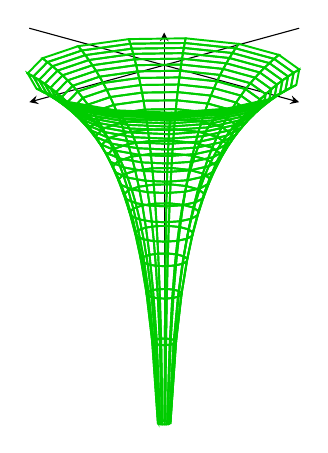
\begin{tikzpicture}
\begin{axis}
[axis lines=center, view={135}{15}, yscale =1.2,
xtick=0, ytick=0, ztick=0, zmax=.5, xmax=1.2, xmin=-1.2, ymax=1.2, ymin=-1.2]

\addplot3[
domain = 0.04 : 0.86,
y domain = 0 : 360,
samples = 24,
samples y = 16, mesh,
draw = green!80!black,
line width = 0.7pt]
({(x*cos(y)},{x*sin(y)},{sqrt(1-x*x)-ln(1/x/x+sqrt(1/x/x-1))});


\end{axis}\end{tikzpicture}
\begin{fig} 유사구면의 형태 \end{fig}
\null\vskip 2em\null
\end{center}
\end{minipage}
%%%%%%%%%%%%%%%%%%%%%%%%%%%%%%%%%%%%%%%%%%%%%%%%%%%%%%%%%%%
%
%              2.1 Upper-half plane Model
%
%%%%%%%%%%%%%%%%%%%%%%%%%%%%%%%%%%%%%%%%%%%%%%%%%%%%%%%%%%%
\subsection{Upper-half plane Model}

위의 회전면을 $w = e^{-u}$, 즉 $\tilde{u} = v, \tilde{v}=w=e^{-u}$로 재매개화하자. 위의 회전면을 다음과 같이 재매개화할 때 제1형식의 변화를 조사하는 것이 목적이다. 이를 위해 다음 정리를 사용하자.
\begin{tcolorbox}[title=재매개화로 인한 제1형식 변화]
Surface patch $\tilde{\boldsymbol{\sigma}}(\tilde{u},\tilde{v})$가 surface patch $\boldsymbol{\sigma}(u,v)$의 재매개화라고, \[ \tilde{E}d\tilde{u}^{2}+2\tilde{F}d\tilde{u}d\tilde{v}+\tilde{G}d\tilde{v}^{2}, \ \ \ \  Edu^{2} + 2Fdudv + Gdv^{2} \]를 각각의 제1형식이라고 가정하자. 그러면 다음이 성립한다.
\begin{enumerate}
    \item $\displaystyle du = \frac{\partial u}{\partial \tilde{u}}d\tilde{u} + \frac{\partial u}{\partial \tilde{v}}d\tilde{v}, dv = \frac{\partial v}{\partial \tilde{u}}d\tilde{u} + \frac{\partial v}{\partial \tilde{v}}d\tilde{v}$ 
    \item $\displaystyle J = \begin{bmatrix}
        \frac{\partial u}{\partial \tilde{u}} & \frac{\partial u}{\partial \tilde{v}} \\
        \frac{\partial v}{\partial \tilde{u}} & \frac{\partial v}{\partial \tilde{v}}
    \end{bmatrix}$라고 한다면, $\begin{bmatrix}\tilde{E} & \tilde{F} \\ \tilde{F} & \tilde{G} \end{bmatrix} = J^{T}\begin{bmatrix}E & F\\F&G \end{bmatrix} J$
\end{enumerate}
\end{tcolorbox}

위의 행렬 $J$를 야코비안(Jacobian)행렬이라고 부른다. $\tilde{u} = v, \tilde{v}=w=e^{-u}$로 재매개화를 수행함을 상기하여 식을 정리하면 $u = -\ln \tilde{v}, v = \tilde{u}$이므로 야코비안 행렬 $J$는 다음과 같다.
\[
J = \begin{bmatrix}
0 & -\frac{1}{\tilde{v}} \\
1 & 0 
\end{bmatrix}
\]
$J$가 가역(invertible)이므로 $(u,v) \mapsto (v,w)$는 재매개화이다. 따라서 $\tilde{E}, \tilde{F}, \tilde{G}$는 다음과 같다. $E = 1, F = 0, G = f^{2}$였으므로,
\begin{align*}
\begin{bmatrix}
\tilde{E} & \tilde{F} \\
\tilde{F} & \tilde{G}
\end{bmatrix} &= J^{T} \begin{bmatrix} E & F \\ F & G \end{bmatrix} J \\
&= \begin{bmatrix}
0 & 1 \\
-\frac{1}{\tilde{v}} & 0 
\end{bmatrix} \begin{bmatrix} E & F \\ F & G \end{bmatrix} \begin{bmatrix}
0 & -\frac{1}{\tilde{v}} \\
1 & 0 
\end{bmatrix} \\
&= \begin{bmatrix}
\frac{1}{w^2} & 0 \\
0 & \frac{1}{w^2}
\end{bmatrix}
\end{align*}
따라서 재매개화된 곡면의 제1형식은 \[\frac{dv^2 + dw^2}{w^2}\]임을 확인할 수 있다. 더하여 $w = e^{-u}$로 정의했기 때문에 $w > 0$이다. 따라서 다음 조건을 만족시키는 반평면에 일정한 음의 가우스 곡률을 지닌 곡면(쌍곡 평면)을 표현할 수 있다.
\begin{tcolorbox}[title=상반 평면 모델(Upper-half plane model)]\[ \mathbb{H}^{2} = \mathbb{H}^{2}(-1) = \{(u, v) \in \mathbb{R}^{2} : v > 0 \},\quad
E=\frac{1}{v^2},~F=0,~G=\frac{1}{v^2}
\]
\end{tcolorbox}
쌍곡 평면을 표현하는 여러 모델 중 상반 평면 모델을 사용하여 쌍곡 평면의 성질들을 알아보자
%%%%%%%%%%%%%%%%%%%%%%%%%%%%%%%%%%%%%%%%%%%%%%%%%%%%%%%%%%%
%
%              2.3 Hyperbolic plane의 성질
%
%%%%%%%%%%%%%%%%%%%%%%%%%%%%%%%%%%%%%%%%%%%%%%%%%%%%%%%%%%%
\subsection{Properties of Hyperbolic plane}
%
%
%%%%%%%%%%%%%%%%%%%%%%%%%%%%%%%%%%%%%%%%%%%%%%%%%%%%%%%%%%%
%            2.3.1 Hyperbolic plane의 곧은선
%%%%%%%%%%%%%%%%%%%%%%%%%%%%%%%%%%%%%%%%%%%%%%%%%%%%%%%%%%%
\begin{tcolorbox}[title=쌍곡 평면의 곧은선(Geodesic)]
쌍곡 평면의 곧은선(geodesic)은 $u$값이 일정한 반직선 $(u,v)=(u_0,t)$, 혹은 중심이 $u$축 위에 있는 반원의 형태 $(u,v)=(u_0+r\tanh{t},r\sech{t})$로 주어진다.
\end{tcolorbox}%
%
\begin{proof}
Geodesic을 만족하기 위한 두 조건으로부터 다음을 알 수 있다.
\begin{align*}
\null&\frac{d}{dt}(E\dot{u}+F\dot{v})=\frac{1}{2}(E_u\dot{u}^2+2F_u\dot{u}\dot{v}+G_u\dot{v}^2)\\
\to~&~%
\frac{d}{dt}(E\dot{u})~=~-\frac{2}{v^3}\dot{u}\dot{v}+\frac{1}{v^2}\Ddot{u}=0
\end{align*}%
\begin{align*}
\null&\frac{d}{dt}(F\dot{u}+G\dot{v})=\frac{1}{2}(E_v\dot{u}^2+2F_v\dot{u}\dot{v}+G_v\dot{v}^2)\\
\to~&~%
\frac{d}{dt}(G\dot{v})~=~\frac{2}{v^3}\dot{v}^2+\frac{1}{v^2}\Ddot{v}=-\frac{2}{2v^3}(\dot{u}^2+\dot{v}^2)\\
\to~&~%
\frac{1}{v^3}(\dot{u}^2-\dot{v}^2)+\frac{1}{v^2}\Ddot{v}=0
\end{align*}
이 직선이 단위 속력이라고 가정하면 $v^2=\dot{u}^2+\dot{v}^2$라는 식을 얻을 수 있다. 여기에서 2번째 식과 3번째 식을 연립해 $u$를 지울 수 있다. 정리하면 다음을 얻는다:
\[
0=\Ddot{v}-2v^{-1}\dot{v}^2+v\quad\to\quad 0=\frac{\Ddot{v}v-2\dot{v}^2}{v^3}+\frac{1}{v}=\frac{d}{dt}\frac{d}{dt}\left(\frac{1}{v}\right)+\frac{1}{v}
\]
따라서 다음의 식이 성립함을 알 수 있다.\[
\displaystyle v=\frac{1}{Ae^{t}+Be^{-t}}=\frac{1}{2\sqrt{AB}}\frac{2}{\frac{\sqrt{A}}{\sqrt{B}}e^{t}+\frac{\sqrt{B}}{\sqrt{A}}e^{-t}}=r\sech(t+\alpha)\quad(r=\frac{1}{2\sqrt{AB}},~e^\alpha=\frac{\sqrt{A}}{\sqrt{B}})
\]%
이를 첫 번째 식에 대입하여 다음을 관찰할 수 있다.\[
0=-\frac{2}{v^3}\dot{u}\dot{v}+\frac{1}{v^2}\Ddot{u}=\frac{d}{dt}\left(\frac{1}{v^2}\right)\dot{u}+\frac{1}{v^2}\frac{d\dot{u}}{dt}=\frac{d}{dt}\left(\frac{\dot{u}}{v^2}\right)\quad\to\quad\dot{u}=Cv^2=r^2C\sech^2(t+\alpha)
\]
이제 unit speed curve 조건을 활용하여 다음을 얻을 수 있다. \[\dot{u}^2=v^2-\dot{v}^2=r^2\sech^2(t+\alpha)(1+\tanh^2(t+\alpha))=r^2\sech^4(t+\alpha)\quad\to\quad C=\frac{1}{r}\]
따라서 $\dot{u}=r\sech^2(t+\alpha)$이고 이를 $t$에 대해 적분하여 $u=r\tanh(t+\alpha)+u_0$라는 결론을 얻을 수 있다. 이는 중심이 $(u_0,0)$인 반원이 된다.
\end{proof}\\[1em]
\begin{minipage}{0.45\textwidth}
앞에서 언급했던 평행선 공준을 다시 살펴보자. Fig 2에서 확인할 수 있듯이, 붉은 색의 곧은선과 만나지 않으며(즉, 평행하며) 붉은 점을 지나는 $u$값이 일정한 직선은 점선의 형태로 존재한다. 하지만, 무수히 많은 반원 꼴의 곧은선 역시 붉은 점을 지나며 붉은 선과 만나지 않으므로 앞에서 언급한 평행선 공준이 성립하지 않음을 확인할 수 있다.
\end{minipage}%
\hfill
\begin{minipage}{0.5\textwidth}
\null\vskip 2em
%
%
%%%%%%%%%%%%%%%%%%%%%%%%%%%%%%%%%%%%%%%%%
%           평행선 공준의 비성립 그림
%%%%%%%%%%%%%%%%%%%%%%%%%%%%%%%%%%%%%%%%%
\begin{center}
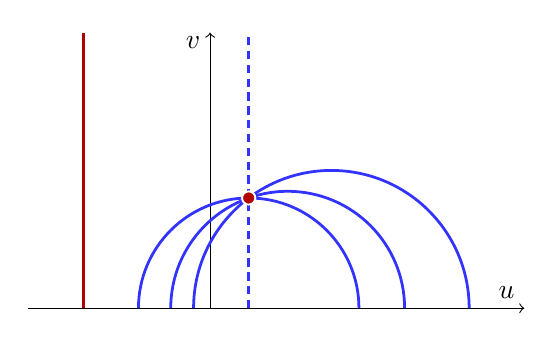
\begin{tikzpicture}[scale=.7]
\draw[->] (-4,0) -- (5,0) node [above left] {$u$}; 
\draw[->] (-.7,0) -- (-.7,5) node [below left] at + (0,0.1) {$v$};
\draw[red!70!black, line width = .1em] (-3,0) -- (-3,5);
\draw[blue!80, line width = .1em] (2,0) arc (0:180:2);
\draw[blue!80, line width = .1em] (4,0) arc (0:180:2.5);
\draw[blue!80, line width = .1em] ({2*sqrt(2)},0) arc (0:180:{3*sqrt(2)/2});
\draw[blue!80, line width = .1em, densely dashed] (0,0) -- (0,5);
\draw[fill=red!70!black, draw=white, line width=.7pt] (0,2) circle [radius=0.12];
\end{tikzpicture}
\begin{fig} 평행선 공준의 비성립 \end{fig}
\null\vskip 2em\null
\end{center}
\end{minipage}

%%%%%%%%%%%%%%%%%%%%%%%%%%%%%%%%%%%%%%%%%%%%%%%%%%%%%%%%%%%
%           2.2.2 Hyperbolic plane의 길이와 각도
%%%%%%%%%%%%%%%%%%%%%%%%%%%%%%%%%%%%%%%%%%%%%%%%%%%%%%%%%%%
\begin{tcolorbox}[title=쌍곡 평면 위의 거리와 각도]
\begin{enumerate}
\item 쌍곡 평면 위의 두 점 $(u_1,v_1)$와 $(u_2,v_2)$의 거리는 다음과 같다.\[
s(t)=\begin{cases}
\ln{v_2}-\ln{v_1} & \text{$u$좌표가 같을 때}\\
\cosh^{-1}\left(1+\displaystyle\frac{(u_2-u_1)^2+(v_2-v_1)^2}{2v_1v_2}\right) & \text{$u$좌표가 같지 않을 때} 
\end{cases}
\]
\item 쌍곡 평면에서의 두 벡터가 이루는 각은 유클리드 평면에서의 각과 값이 같다.
\end{enumerate}
\end{tcolorbox}
\begin{proof}
길이의 경우 다음의 두 경우로 나누어 살펴보아야 한다.
\begin{enumerate}
\item $u$좌표가 같을 때:\\
이 경우 곧은선이 $v$축과 평행한 직선이기 때문에 다음과 같이 구할 수 있다.\[
s(t)=\int_{t_1}^{t_2}\sqrt{\frac{\dot{u}^2+\dot{v}^2}{v^2}}dt=\int_{t_1}^{t_2}\frac{1}{t}dt=\ln{t_2}-\ln{t_1}=\ln{v_2}-\ln{v_1}
\]
\item $u$좌표가 같지 않을 때:\\
이 경우 곧은선이 중심이 $u$축 위에 있는 반원 꼴이기 때문에 다음과 같이 구할 수 있다.
\begin{align*}
\!\!\!\!\!\!\!\!\!\!\!\!\!\!%
s(t)&=\int_{t_1}^{t_2}\sqrt{\frac{\dot{u}^2+\dot{v}^2}{v^2}}dt
=\int_{t_1}^{t_2}\sqrt{\frac{r^2\sech^2{t}(\sech^2{t}+\tanh^2{t})}{r^2\sech^2{t}}}dt=\int_{t_1}^{t_2}1dt
=t_2-t_1\\
&=\cosh^{-1}(\cosh(t_2-t_1)) = \cosh^{-1}(\cosh(t_2)\cosh(t_1)-\sinh(t_2)\sinh(t_1))\\
&=\cosh^{-1}\left(\frac{r^2}{v_1v_2}\left(1-\frac{x_1-x_0}{r}\frac{x_2-x_0}{r}\right)\right)
=\cosh^{-1}\left(\frac{1}{v_1v_2}(r^2-(u_1-u_0)(u_2-u_0))\right)\\
&=\cosh^{-1}\left(\frac{1}{2v_1v_2}((u_1-u_0)^2+(u_2-u_0)^2+v_1^2+v_2^2-2(u_1-u_0)(u_2-u_0))\right)\\
&=\cosh^{-1}\left(\frac{1}{2v_1v_2}((u_1-u_0-u_2+u_0)^2+v_1^2+v_2^2)\right)=\cosh^{-1}\left(1+\displaystyle\frac{(u_2-u_1)^2+(v_2-v_1)^2}{2v_1v_2}\right)
\end{align*}
\end{enumerate}
$(u,v)$에서 두 벡터 $w_1=(w_{1u},w_{1v})$와 $w_2=(w_{2u},w_{2v})$의 내적 $\langle w_1,w_2\rangle$ 는 다음과 같이 표현할 수 있다.\[
\langle w_1,w_2\rangle=\frac{w_{1u}w_{2u}+w_{1v}w_{2v}}{v^2}
\]
따라서 각을 다음과 같이 구할 수 있다.\[
\cos\theta=\frac{\langle w_1,w_2\rangle}{\sqrt{\langle w_1,w_1\rangle\langle w_2,w_2\rangle}}=\frac{w_{1u}w_{2u}+w_{1v}w_{2v}}{\sqrt{w_{1u}^2+w_{1v}^2}\sqrt{w_{2u}^2+w_{2v}^2}}
\]
이는 평면에서의 $\cos$ 값과 정확히 일치하므로 쌍곡 평면에서 두 벡터가 이루는 각은 유클리드 평면에서의 각과 같은 값임을 알 수 있다.
\end{proof}


\newpage
\section{Lorentz plane/space}
\subsection{Distance of Lorentz plane/space using metric and IBF}
먼저 metric tensor(이하 metric)의 정의를 살펴보자. 이전에 배웠던 쌍선형형식(bilinear form)과 다양체(manifold)의 정의, 접공간(tangent space)에 대한 정의들을 상기하자.
\begin{tcolorbox}[title=Metric]
$M$을 $n$차원 매끄러운 다양체(smooth manifold)라고 하자. $\mathbf{p} \in M$에서 정의된 접공간(tangent space)을 $T_{\mathbf{p}}M$라 하자.\\
이때 metric은 다음 세 조건을 만족하는 함수 $g_{\mathbf{p}} : T_{\mathbf{p}}M \times T_{\mathbf{p}}M \to \mathbb{R}$이다.
\begin{enumerate}
\item $g_{\mathbf{p}}$는 bilinear하다. 즉, $\mathbf{x}, \mathbf{y}, \mathbf{z} \in T_{\mathbf{p}}M$과 $a, b \in \mathbb{R}$에 대하여 다음이 성립한다.
\begin{align*}
    g_{\mathbf{p}}(a\mathbf{x}+b\mathbf{y}, \mathbf{z}) &= ag_{\mathbf{p}}(\mathbf{x}, \mathbf{z}) + bg_{\mathbf{p}}(\mathbf{y}, \mathbf{z}) \\
    g_{\mathbf{p}}(\mathbf{x}, a\mathbf{y} + b\mathbf{z}) &= ag_{\mathbf{p}}(\mathbf{x}, \mathbf{y}) + bg_{\mathbf{p}}(\mathbf{x}, \mathbf{z})
\end{align*}
\item $g_{\mathbf{p}}$는 symmetric하다. 즉, $\mathbf{x}, \mathbf{y} \in T_{\mathbf{p}}M$에 대하여 다음이 성립한다.
\[ g_{\mathbf{p}}(\mathbf{x}, \mathbf{y}) = g_{\mathbf{p}}(\mathbf{y}, \mathbf{x}) \]
\item $g_{\mathbf{p}}$는 nondegenerate하다. 즉, 모든 $\mathbf{x} \in T_{\mathbf{p}}M, \mathbf{x} \neq \mathbf{0}$에 대하여, $g_{\mathbf{p}}(\mathbf{x}, \mathbf{y}) \neq 0$이 되는 $\mathbf{y} \in T_{\mathbf{p}}M$가 존재한다.
\end{enumerate}
\end{tcolorbox}
유클리드 공간의 내적으로부터 길이와 각도를 정의한 것처럼, metric은 일반적인 공간, 더 나아가 다양체에 대하여 길이와 각도를 정의할 수 있게 한다.
예를 들어, 일반적인 2차원 유클리드 평면, 그 중 데카르트 좌표(cartesian coordinate)로 나타내는 경우의 metric은 다음과 같이 주어진다.
\[g = \begin{bmatrix}1&0\\0&1\end{bmatrix}\]
이 metric을 $ds^{2} = dx^{2} + dy^{2}$과 같은 형태로 쓰기도 한다. 극좌표(polar coordinate)의 metric은 위의 metric에 야코비안 행렬을 사용하여 변수변환을 진행하면 얻어진다.
\[g' = J^{T}gJ = \begin{bmatrix}\cos \theta&\sin \theta \\-r\sin \theta&r\cos \theta\end{bmatrix} \begin{bmatrix}1&0\\0&1\end{bmatrix} \begin{bmatrix}\cos \theta&-r\sin \theta\\\sin \theta &r\cos \theta\end{bmatrix} = \begin{bmatrix}1&0\\0&r^{2}\end{bmatrix}\]
이 경우 metric은 $ds^{2} = dr^{2} + r^2d\theta^{2}$으로도 쓰기도 한다. $\mathbb{R}^{3}$위의 단위 구면에서 정의되는 구면 좌표계의 경우의 metric은 다음과 같이 쓸 수 있다.
\[g = \begin{bmatrix}1&0\\0&\sin ^{2}\theta\end{bmatrix}\]
마찬가지로, 이 경우의 metric은 $ds^{2} = d\theta^{2} + \sin^{2}\theta d\varphi^{2}$의 형태로 쓰기도 한다. 즉 metric은 우리에게 익숙한 $E, F, G$행렬의 개념을 일반화한 것이라고 생각할 수 있다.
\begin{tcolorbox}[title=Lorentz 평면/공간의 metric]
Lorentz 평면/공간은 metric을
\[ g = \begin{bmatrix} 1 & 0 & \cdots & 0 \\ 0 & 1 & \cdots & 0 \\ \vdots & \vdots & \ddots & \vdots \\
0 & 0 & \cdots & -1 \end{bmatrix}\]
로, 즉 \[ds^2=dx_1^2+dx_2^2+\cdots +dx_{n-1}^2-dt^2\]의 형태로 준 공간을 말한다. $n=2$일 때를 Lorentz 평면이라고 한다.
\end{tcolorbox}
Lorentz 평면에서도 두 점 사이의 거리를 $\mathbb{E}^n$에서 정의하는 방식과 같은 방식으로 부여할 수 있다. Lorentz 평면은 $E=1, F=0, G=-1$을 만족하고 $EG-F^2=-1$이므로, $E, F, G$ 행렬이 양의 준정부호(positive semidefinite, 이하 PSD)가 아닌 것을 알 수 있다. 즉, 쌍선형형식이 정부호가 아니다(Indefinite Bilinear Form, 이하 IBF). 유클리드 공간에서의 거리가 유클리드 공간에서의 내적으로부터 나오고, 내적은 PSD를 만족시킴을 상기해보자. 따라서, Lorentz평면에서의 거리는 일반적으로 다루는 거리와 여러 면에서 다른 특성을 가진다. Lorentz 공간의 경우, $t$를 제외하면 일반적인 $\mathbb{R}^{n-1}$에서의 거리와 같으므로 Lorentz 평면에서만 생각해도 충분하다. 이 경우에 대해 살펴보자.
\begin{tcolorbox}[title=Lorentz 평면에서의 거리]
Lorentz 평면에서 거리는 $b=\sqrt{(x_a-x_b)^2-(t_a-t_b)^2}$의 형태이고, 일반적인 거리와는 아래와 같은 차이를 보인다.
\begin{enumerate}
\item 거리는 실수가 아닐 수 있다. $(b((0,0),(0,1))=i)$
\item 서로 다른 두 점 사이의 거리는 0일 수도 있다. $(b((1,0),(0,1))=0)$
\end{enumerate}
\end{tcolorbox}
Lorentz 평면/공간에서의 거리는 일반적인 의미에서의 거리와 다르다는 점에 주의하자.

\subsection{Geodesic of Lorentz plane}

\begin{tcolorbox}[title=Lorentz 평면에서의 곧은선]
Lorentz 평면에서의 곧은선은 다음과 같은 형태로 주어진다.
\\$\gamma(p)=ax(p)t(p)+bx(p)+ct(p)+d \quad (a,b,c,d\in \mathbb{R})$
\end{tcolorbox}
\begin{proof}
Geodesic을 만족하기 위한 두 조건과 Lorentz 평면의 $E, F, G$로부터 다음을 알 수 있다.
\[\frac{d}{dp}(\dot{x})=0, \frac{d}{dp}(-\dot{t})=0\quad \to \quad \Ddot{x}=0,\Ddot{t}=0\]
위의 미분방정식을 연립하여 풀면 geodesic의 형태를 쉽게 확인할 수 있다. 
\end{proof}
%%%%%%%%%%%%%%%%%%%%%%%%%%%%%%%%%%%%%%%%%%%%%%%%%%%%%%%%
%
% 리지드 모션이 뭔 좆소리임 용어를 정의하고 써봐
%
%%%%%%%%%%%%%%%%%%%%%%%%%%%%%%%%%%%%%%%%%%%%%%%%%%%%%%%%
\subsection{Lorentz transformation}
Lorentz 평면의 성질을 지니고 있는 metric은 유지하며, 동시에 변수변환을 진행하는 상황을 생각해보자. 이전에 정의했던 야코비안 행렬을 상기하자.
\begin{tcolorbox}[title = Lorentz 군]
Lorentz 평면의 metric이 $\varepsilon = \begin{bmatrix} 1 & 0 \\ 0 & -1\end{bmatrix}$로 주어져 있다고 하자.
\begin{itemize}
    \item Lorentz 군: $O(1, 1) = \{ M \in \mathbb{R}^{2 \times 2} \mid M\varepsilon M^T = \varepsilon\}$
    \item 특수 Lorentz 군: $SO(1, 1)^+ = \{ M \in \mathbb{R}^{2 \times 2} \mid M\varepsilon M^T = \varepsilon, \det M = 1, \text{tr } M > 0\}$
\end{itemize}
\end{tcolorbox}


즉, Lorentz 군은 Lorentz 평면의 metric을 Lorentz 평면의 metric으로 보내는 야코비안 행렬들의 모임이고, 특수 Lorentz 군은 이 중에서 행렬식의 값이 $1$이고 주대각합이 $0$보다 큰 행렬들의 모임이라고 할 수 있다. 여기에서 Lorentz 군의 원소를 Lorentz 변환, 특수 Lorentz 군의 원소를 특수 Lorentz 변환이라고 한다.

\begin{tcolorbox}[title=Lorentz 변환의 형태\null]
일반적인 Lorentz 변환의 형태는 아래와 같다.\[
\begin{bmatrix}
    \alpha \cosh{\phi} & \beta \sinh{\phi}\\
    \beta \sinh{\phi} & \alpha \cosh{\phi}
\end{bmatrix} = \begin{bmatrix}
    \alpha & 0 \\
    0 & \beta 
\end{bmatrix}\begin{bmatrix}
    \cosh{\phi} & \sinh{\phi}\\
    \sinh{\phi} & \cosh{\phi}
\end{bmatrix}\quad(\alpha, \beta \in \{-1, 1\},~\phi \in \mathbb{R})
\]
특수 Lorentz 변환은 $\alpha = 1, \beta = 1$인 경우이다.
\end{tcolorbox}

\begin{tcolorbox}[title=Poincaré 변환]
Poincaré 변환은 $x, t$에 대한 다음과 같은 변환이다. ($M \in O(1, 1)$)
\[\begin{bmatrix}
    x \\ t
\end{bmatrix} \mapsto M\begin{bmatrix}
    x \\ t
\end{bmatrix} + \begin{bmatrix}
    x_0 \\ t_0
\end{bmatrix}\]
이 변환은 Lorentz metric을 보존하는 변환이다.
\end{tcolorbox}
\begin{proof}
여기서는 특수 Lorentz 변환의 경우만 계산한다.
\begin{align*}
    \begin{bmatrix}
        \tilde{x} \\ \tilde{t}
    \end{bmatrix} &= \begin{bmatrix}
        \cosh{\phi} & \sinh{\phi}\\
        \sinh{\phi} & \cosh{\phi}
    \end{bmatrix}\begin{bmatrix}
        x \\ t
    \end{bmatrix}\\
    \begin{bmatrix}
        x \\ t
    \end{bmatrix} &= \begin{bmatrix}
        \cosh{\phi} & -\sinh{\phi}\\
        -\sinh{\phi} & \cosh{\phi}
    \end{bmatrix}
    \begin{bmatrix}
        \tilde{x} \\ \tilde{t} 
    \end{bmatrix}
\end{align*}
\begin{align*}
    dx^2 - dt^2 &= \begin{bmatrix}
        dx & dt
    \end{bmatrix}
    \begin{bmatrix}
        1 & 0\\0 & -1
    \end{bmatrix}
    \begin{bmatrix}
        dx \\ dt
    \end{bmatrix}\\
    &= \begin{bmatrix}
        d\tilde{x} & d\tilde{t}
    \end{bmatrix}
    \begin{bmatrix}
        \cosh{\phi} & -\sinh{\phi}\\
        -\sinh{\phi} & \cosh{\phi}
    \end{bmatrix}
    \begin{bmatrix}
        1 & 0\\0 & -1
    \end{bmatrix}
    \begin{bmatrix}
        \cosh{\phi} & -\sinh{\phi}\\
        -\sinh{\phi} & \cosh{\phi}
    \end{bmatrix}
    \begin{bmatrix}
        d\tilde{x} \\ d\tilde{t}
    \end{bmatrix}\\
    &=\begin{bmatrix}
        d\tilde{x} & d\tilde{t}
    \end{bmatrix}
    \begin{bmatrix}
        1 & 0\\
        0 & -1
    \end{bmatrix}
    \begin{bmatrix}
        d\tilde{x} \\ d\tilde{t}
    \end{bmatrix} = d\tilde{x}^2 - d\tilde{t}^2
\end{align*}
\end{proof}
\subsection{Relation between Hyperbolic plane and 3-dimensional Lorentz space}

3차원 Lorentz 공간에서 원점과의 거리가 $i$이면서 $t>0$인 $\mathbb{H}$는 아래 figure에 있는 붉은 쌍곡면이다. 이를 $(0,0,-1)$을 기준으로 $xy-$plane에 사영을 하면 이는 $B_1(0,0)$에 들어가게 되고 이를 $(u,v)$로 두었을 때 다음과 같이 $\boldsymbol{\sigma}$가 정의된다.%
\[
(x,y,t)=\boldsymbol{\sigma}(u,v)=\left( \frac{2u}{1-u^{2}-v^{2}}, \frac{2v}{1-u^{2}-v^{2}}, \frac{1+u^{2}+v^{2}}{1-u^{2}-v^{2}} \right)
\]
이를 $u$와 $v$로 미분하면 다음과 같은 식이 나온다:%
\begin{align*}
\boldsymbol{\sigma}_u &= \frac{2}{(1-u^{2}-v^{2})^{2}}(1+u^{2}-v^{2},2uv,2u),\\
\boldsymbol{\sigma}_v &= \frac{2}{(1-u^{2}-v^{2})^{2}}(2uv,1-u^{2}+v^{2},2v).
\end{align*}
이를 통해 $E,F,G$를 구하면 다음과 같이 나온다:\[
E=\frac{4}{(1-u^{2}-v^{2})^{2}},~F=0,~G=\frac{4}{(1-u^{2}-v^{2})^{2}}
\]
$E,F,G$를 구할 때 Lorentz 공간의 metric을 적용하여 구함에 유의하자. 이 모델은 푸엥카레 원반 모델(Poincaré disk model)이라고 불리는데 이는 우리가 다룬 표현이 아니다. $(u',v')=f(u,v)=\left(\frac{-2v}{(u-1)^2+v^2},\frac{1-u^2-v^2}{(u-1)^2+v^2}\right)$라는 변환을 생각해 보자. 치환적분을 사용하기 위해 각 성분으로 편미분하면 다음과 같다.
\begin{align*}
f_u&=\left(
\frac{4(u-1)v}{((u-1)^2+v^2)^2},
\frac{-2u((u-1)^2+v^2)+2(u-1)(1-u^2-v^2)}{((u-1)^2+v^2)^2}\right)\\
&=\left(
\frac{4(u-1)v}{((u-1)^2+v^2)^2},
\frac{2(u-1)^2-2v^2}{((u-1)^2+v^2)^2}\right)\\
f_v&=\left(
\frac{-2((u-1)^2+v^2)+4v^2}{((u-1)^2+v^2)^2},
\frac{-2v((u-1)^2+v^2)-2v(1-u^2-v^2)}{((u-1)^2+v^2)^2}\right)\\
&=\left(
\frac{2v^2-2(u-1)^2}{((u-1)^2+v^2)^2},
\frac{4(u-1)v}{((u-1)^2+v^2)^2}\right)
\end{align*}
\begin{align*}
f_u\cdot f_u&=\frac{(4(u-1)v)^2 + (2(u-1)^2-2v^2)^2}{((u-1)^2+v^2)^4}=\frac{4}{((u-1)^2+v^2)^2}\\
f_u\cdot f_v&=\frac{4(u-1)v(2(u-1)^2-2v^2+2v^2-2(u-1)^2)}{((u-1)^2+v^2)^4}=0\\
f_v\cdot f_v&=\frac{(4(u-1)v)^2 + (2v^2-2(u-1)^2)^2}{((u-1)^2+v^2)^4}=\frac{4}{((u-1)^2+v^2)^2}\\
\end{align*}
이를 통해 $[f_u~f_v]$ 행렬의 determinant가 $\frac{4}{((u-1)^2+v^2)^2}$이고, 다음이 성립함을 알 수 있다.\[
\begin{bmatrix}
E' & F'\\F' & G'
\end{bmatrix}
=
\begin{bmatrix}
f_u & f_v
\end{bmatrix}^{-T}
\begin{bmatrix}
E & F\\F & G
\end{bmatrix}
\begin{bmatrix}
f_u & f_v
\end{bmatrix}^{-1}
=
\begin{bmatrix}
\frac{((u-1)^2+v^2)^2}{(1-u^2-v^2)^2} & 0\\0 & \frac{((u-1)^2+v^2)^2}{(1-u^2-v^2)^2}
\end{bmatrix}
=
\begin{bmatrix}
1/v'^2 & 0\\0 & 1/v'^2
\end{bmatrix}
\]
%bro.
위에서 $-T$의 경우 역행렬의 transpose를 축약한 기호이다. 따라서 우리가 처음에 정의했던 $E,F,G$와 동일해짐을 확인할 수 있다. 이를 그림으로 표현한 것이 아래 figure이다. 두개의 쌍곡 평면 모델들의 경우 복소평면처럼 생각할 수 있고, 이를 변환한 함수를 적어두었다.
%%%%%%%%%%%%%%%%%%%%%%%%%%%%%%%%%%%%%%%%%%%%%%%
%    Lorentz 공간의 atlas와 쌍곡 평면과의 관계
%%%%%%%%%%%%%%%%%%%%%%%%%%%%%%%%%%%%%%%%%%%%%%%
\begin{center}
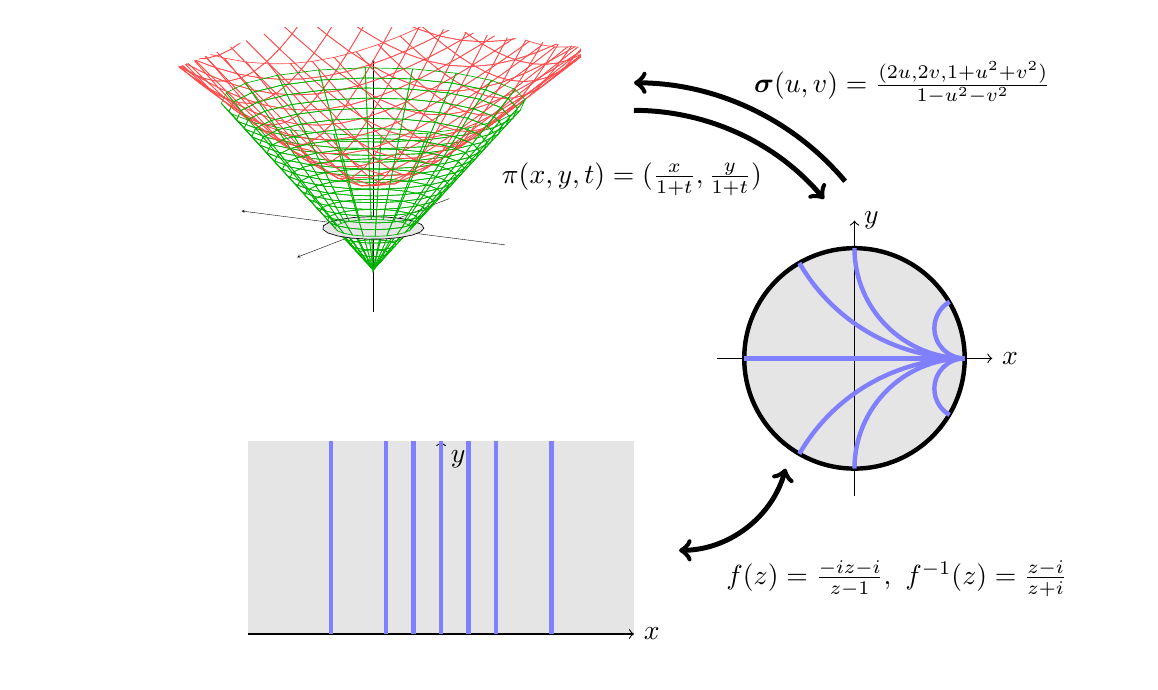
\begin{tikzpicture}[scale = .35]
\clip (-5,-11) rectangle (35,12);
\begin{axis}
[view={210}{15},axis lines=center, xtick=\empty, ytick=\empty, ztick=\empty,
xmin = -3, ymin = -3, zmin=-2, xmax = 3, ymax = 3, zmax=4, scale=2.2]


\addplot3[domain = 0 : 1, y domain = 0 : 360,
samples = 6, samples y = 20, mesh,
draw = green!70!black, line width = 0.7pt]
({x*3/4*cos(y)},{x*3/4*sin(y)},{x-1});

\addplot3[domain = 0 : 360,
samples = 20, fill=gray!20, line width = 0.7pt]
({cos(x)},{sin(x)},{0});

\addplot3[domain = 1 : 4, y domain = 15 : 195,
samples = 16, samples y = 11, mesh,
draw = green!70!black, line width = 0.7pt]
({x*3/4*cos(y)},{x*3/4*sin(y)},{x-1});

\addplot3[domain = -5 : 5, y domain = -5 : 5,
samples = 21, samples y = 21, mesh,
draw = red!70, line width = 0.7pt]
({x},{y},{sqrt(x^2+y^2+1)});

\addplot3[domain = 1 : 4, y domain = 195 : 375,
samples = 16, samples y = 11, mesh,
draw = green!70!black, line width = 0.7pt]
({x*3/4*cos(y)},{x*3/4*sin(y)},{x-1});
\end{axis}

%
%
%

\draw[ultra thick, fill=gray!20] (25,0) circle [radius=4];
\draw[->] (20,0) -- (30,0) node [right] {$x$};
\draw[->] (25,-5) -- (25,5) node [right] {$y$};
\draw[blue!50, ultra thick] (29,0) arc (270 : 210 : 1.732*4);
\draw[blue!50, ultra thick] (29,0) arc (270 : 180 : 4);
\draw[blue!50, ultra thick] (29,0) arc (270 : 120 : 1.1);
\draw[blue!50, ultra thick] (21,0) -- (29,0);
\draw[blue!50, ultra thick] (29,0) arc (90 : 150 : 1.732*4);
\draw[blue!50, ultra thick] (29,0) arc (90 : 180 : 4);
\draw[blue!50, ultra thick] (29,0) arc (90 : 240 : 1.1);

%
%
%

\draw[fill=gray!20,draw=none] (3,-10) rectangle (17,-3);
\draw[->] (3,-10) -- (17,-10) node [right] {$x$};
\draw[->] (10,-10) -- (10,-3) node [below right] {$y$};
\foreach \i in {-4,-2,-1,0,1,2,4}
\draw[blue!50, ultra thick] (\i+10,-10) -- (\i+10,-3);

%
%
%

\draw[line width = 0.18em, <-] (17,10) arc (90 : 40 : 10);
\node[right] at (21,10) {$\boldsymbol{\sigma}(u,v)=\frac{(2u,2v,1+u^2+v^2)}{1-u^{2}-v^{2}}$};

\draw[line width = .18em, ->] (17,9) arc (90 : 40 : 9);
\node[left] at (22,6.5) {$\pi(x,y,t)=(\frac{x}{1+t},\frac{y}{1+t})$};

%
%
%

\draw[line width = .18em, <->] (22.5,-4) arc (-15 : -90 : 4);
\node[right] at (20,-8) {$f(z)=\frac{-iz-i}{z-1},~f^{-1}(z)=\frac{z-i}{z+i}$};

%
%
%

\end{tikzpicture}
\begin{fig} Lorentz 공간의 atlas와 쌍곡 평면과의 관계\end{fig}
\end{center}
%이걸 어케 써야할지 후...
%양성덕의 미분 기하학 제 7장의 제일 첫 장에 뫼비우스 변환이 나와있음
%먼저 그걸 소개하자.
%그리고 뫼비우스 변환의 보조정리들(7.0.2)을 모두 증명하자.
%7.9 쌍곡 평면의 여러 모델들에 그림이 나와있는데, 이를 통해 기하학적 직관을 심어주자
%isometry 보고서에 있는거 다 증명 적기
%11.3에 poincare disc와 쌍곡 평면 사이 isometry 내용 나와있음
\newpage
\section{Special theory of relativity}
\subsection{Representation of space and time through Lorentz plane/space}
특수 상대성 이론에서는 시공간을 Lorentz 평면/공간의 형태로 표현한다. $n$차원 시공간에 대해서 $n-1$차원의 공간을 $x_1,x_2,\dots,x_{n-1}$의 변수로, 시간을 $t$로 나타낸다. 이 보고서는 2차원 시공간에 한해 다루고자 하므로, Lorentz 평면을 중점적으로 살펴보고자 한다.
\begin{tcolorbox}[title=Lorentz 평면에서의 벡터의 구분]
Lorentz 평면의 벡터들은 원점과의 IBF의 제곱으로 다음과 같이 구분한다.
    \begin{itemize}
        \item light-like vector ($\{b(0,\overrightarrow{v})\}^2=0$)
        \item space-like vector ($\{b(0,\overrightarrow{v})\}^2>0$)
        \item time-like vector ($\{b(0,\overrightarrow{v})\}^2<0$)
    \end{itemize}
\end{tcolorbox}
후술할 특수 상대성 이론은 그 두 번째 가정에서 빛의 속력을 어느 관성계에서나 일정하도록 두게 되는데, 이는 light-like vector를 $|\frac{dx}{dt}|=1$인 것으로, 즉 빛의 속력을 1로 설정한 것이다. 또한, 모든 물체의 속도 벡터는 공간적 벡터에 속하지 않는데, 이는 물체의 속도가 빛의 속도를 넘지 못한다는 아인슈타인의 생각이 반영된 것이다.

\subsection{Relative speed on uniform velocity motion}
관찰자 $O$와 $O$에서 일정한 속도 $v$로 멀어지고 있는 관찰자 $\widetilde{O}$를 생각하자.
$O$의 시각에서 $O$, $\widetilde{O}$가 관찰한 사건 $p$의 위치와 시간을 각각 $x, t$, $\tilde{x}, \tilde{t}$라고 하자.
특수 상대성 이론이 밝히고자 하는 바는 이 $x, t, \tilde{x}, \tilde{t}$의 관계이다.

아래는 아인슈타인이 주장한 특수 상대성 이론의 가정이다.
\begin{tcolorbox}[title=특수 상대성 이론에서의 가정\null]
\begin{enumerate}
    \item 모든 관성계(inertial frame)는 동등하다.
    \item 빛의 속력은 어느 관성계에서나 일정하다.
\end{enumerate}
\end{tcolorbox}
첫 번째 가정을 수학적으로 표현하면 '모든 관성계의 metric 표현 식은 같은 꼴이다'가 된다. 앞서 Lorentz 공간의 metric이 $ds^2 = dx^2 - dt^2$로 표현된다고 하였으니 $xt$-공간에서는 $dx^2 - dt^2$가, $\tilde{x}\tilde{t}$-공간에서는 $d\tilde{x}^2 - d\tilde{t}^2$가 metric이 된다. 여기서 $xt$-공간에서 $\tilde{x}\tilde{t}$-공간으로, 또는 그 반대로 바꾸는 변환은 metric을 보존하는 변환이므로 상술한 Poincaré 변환이 된다.

우선 특수 Lorentz 변환을 적용하자.
\[
    \begin{bmatrix}
        \tilde{x}\\\tilde{t}
    \end{bmatrix} = 
    \begin{bmatrix}
        \cosh{\phi} & \sinh{\phi}\\
        \sinh{\phi} & \cosh{\phi}
    \end{bmatrix}
    \begin{bmatrix}
        x \\ t
    \end{bmatrix}, \quad \phi \in \mathbb{R}
\]

$\widetilde{O}$의 관성계에서 자기 자신은 고정된 채로 시간만 흐르게 된다. $\widetilde{O}$가 관찰하는 자기 자신의 궤적을 매개변수 $s$를 활용해 $\tilde{x}(s) = 0$, $\tilde{t}(s) = s$로 표현할 수 있는데, 이를 대입하면
\[
    \begin{bmatrix}
        x(s) \\ t(s)
    \end{bmatrix} =
    \begin{bmatrix}
        \cosh{\phi} & -\sinh{\phi}\\
        -\sinh{\phi} & \cosh{\phi}
    \end{bmatrix}
    \begin{bmatrix}
        0 \\ s
    \end{bmatrix}
\]
$x(s) = -\sinh{\phi} \cdot s$, $t(s) = \cosh{\phi} \cdot s$를 얻는다.
따라서 $O$가 보는 $\widetilde{O}$의 속도는 $v = -\tanh{\phi}$이다.
%
%
%%%%%%%%%%%%%%%%%%%%%%%%%%%%%%%%%%%%%%%%%
%       Lorentz 변환의 예시 : 7:24:25
%%%%%%%%%%%%%%%%%%%%%%%%%%%%%%%%%%%%%%%%%
\begin{center}
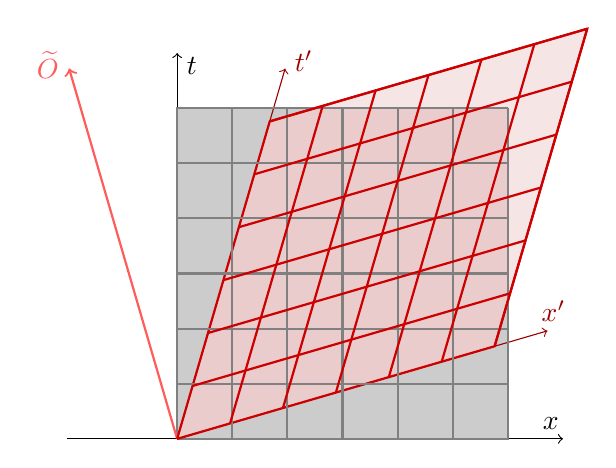
\begin{tikzpicture}[scale=.7]
\draw[->] (-2,0) -- (7,0) node [above left] at + (0.1,0) {$x$}; 
\draw[->] (0,0) -- (0,7) node [below right] at + (0,0.1) {$t$};
\draw[fill=black!20,thick,draw=black!50] (0,0) -- (6,0) -- (6,6) -- (0,6) -- (0,0);
\fill[red!60!black!20!white] (0,0) --  (1.68,5.76) -- (2.5,6) --  (6,6) --  (6,2.5) -- (5.76,1.68) -- (0,0);
\fill[red!60!black!10!white] (2.5,6) --  (6,6) --  (6,2.5) -- ({5.76+1.68},{1.68+5.76}) -- (2.5,6);

\draw[thick,->,red!100!black!64] (0,0) -- (-1.96,6.72) node [below left] at + (0,0.5) {$\widetilde{O}$};

\draw[->,red!60!black] (0,0) -- (6.72,1.96) node [above left] at + (0.5,0) {$x'$}; 
\draw[->,red!60!black] (0,0) -- (1.96,6.72) node [below right] at + (0,0.5) {$t'$};
\draw[thick,draw=red!80!black] (0,0) --  (1.68,5.76) -- ({5.76+1.68},{1.68+5.76}) --  (5.76,1.68) --  (0,0);
\foreach \i in {1,2,3,4,5,6}{
\draw[black!50,thick] (\i,0) -- (\i,6);
\draw[black!50,thick] (0,\i) -- (6,\i);
}
\foreach \i in {1,2,3,4,5,6}{
\draw[red!80!black,thick] (\i*0.96,\i*0.28) --  + (1.68,5.76);
\draw[red!80!black,thick] (\i*0.28,\i*0.96) --  + (5.76,1.68);
}
\end{tikzpicture}
\begin{fig} $v = -\frac{7}{24}$의 경우. $O$가 보는 $\widetilde{O}$의 움직임과 $\widetilde{O}$ 시점의 관성계\end{fig}
\end{center}

\subsection{Facts from Special theory of relativity}
\subsubsection{Speed of every object is smaller than 1}
특수 Lorentz 변환을 살펴보자. 관찰자 $O(x, t)$와 입자 $P(\tilde{x}, \tilde{t})$에 대해,
\[
    \begin{bmatrix}
        \tilde{x}\\\tilde{t}
    \end{bmatrix} = 
    \begin{bmatrix}
        \cosh{\phi} & \sinh{\phi}\\
        \sinh{\phi} & \cosh{\phi}
    \end{bmatrix}
    \begin{bmatrix}
        x \\ t
    \end{bmatrix}, \quad \phi \in \mathbb{R}
\]
였다. 앞서 구한 바에 따라 입자의 속도는 $v = -\tanh(\phi)$이므로, 입자의 속력은 다음과 같이 표현된다.
\begin{equation*}
|\!|v|\!| = |\!|-\tanh(\phi)|\!|<1
\end{equation*}
따라서 입자의 속력 $v$는 항상 1보다 작아야 한다.

\subsubsection{The speed of light is 1 in all inertial frame}
특수 상대성 이론의 두 번째 공리는 빛의 속력이 어느 관성계에서나 같다는 것이었다. 이를 Lorentz 변환을 통해서 재확인할 수 있다.

두 사건 $(t_1, x_1)$과 $(t_2, x_2)$가 빛에 의해 연결되어 있다면 그 metric은
\begin{equation*}
(t_2 - t_1)^2 - (x_2 - x_1)^2 = 0
\end{equation*}
이고, Lorentz 변환 하에서도 이 관계가 유지된다(이는 $x$와 $t$가 같은 비율로 변화하기 때문이다). 따라서 모든 관성계에서 빛의 속력은 $dx/dt = 1$로 항상 일정함을 알 수 있다.

\subsubsection{Simultaneous event is relative}
두 관성계 $S$와 $S'$를 고려하자. $S$에서 두 사건이 동시에 일어난 것을 $t_1 = t_2$로 표현할 수 있다. 그러나 $S'$에서 보는 두 사건에는 다음과 같이 시간 차이 $\tilde{t}_1 \neq \tilde{t}_2$가 발생한다:
\[
    \begin{bmatrix}
        \tilde{x}_1\\\tilde{t}_1
    \end{bmatrix} = 
    \begin{bmatrix}
        \cosh{\phi} & \sinh{\phi}\\
        \sinh{\phi} & \cosh{\phi}
    \end{bmatrix}
    \begin{bmatrix}
        x_1 \\ t_1
    \end{bmatrix}
\]
\[
    \begin{bmatrix}
        \tilde{x}_2\\\tilde{t}_2
    \end{bmatrix} = 
    \begin{bmatrix}
        \cosh{\phi} & \sinh{\phi}\\
        \sinh{\phi} & \cosh{\phi}
    \end{bmatrix}
    \begin{bmatrix}
        x_2 \\ t_2
    \end{bmatrix}
\]
\[
    \begin{cases}
        \tilde{x}_1 = \cosh{\phi}\cdot x_1 + \sinh{\phi}\cdot t_1\\
        \tilde{t}_1 = \sinh{\phi}\cdot x_1 + \cosh{\phi}\cdot t_1
    \end{cases}
\]
\[
    \begin{cases}
        \tilde{x}_2 = \cosh{\phi}\cdot x_2 + \sinh{\phi}\cdot t_2\\
        \tilde{t}_2 = \sinh{\phi}\cdot x_2 + \cosh{\phi}\cdot t_2
    \end{cases}
\]
따라서, $\tilde{t}_1 \neq \tilde{t}_2$일 수 있다. 이는 한 관찰자의 입장($S$)에서 동시에 일어난 사건이 다른 관찰자의 입장에서는 동시에 일어나지 않을 수 있음을 의미한다.

\subsubsection{Time expansion occurs}
시간 팽창은 한 관찰자의 입장에서 시차를 두고 발생한 두 사건이 상대적으로 움직이는 관찰자에게 더 긴 시차를 두고 발생하는 현상이다.

Lorentz 변환에 따르면,
\begin{equation*}
\tilde{t} = \cosh(\phi) t + \sinh(\phi) x
\end{equation*}
이다($\sinh(\phi)$와 $x$의 부호가 같다). 따라서 움직이는 관찰자는 정지한 관찰자에 비해 시간이 더 천천히 흐르는 것으로 보인다.

특히 같은 장소에서 발생한 사건의 경우 $x = 0$이므로,
\begin{equation*}
\tilde{t} = \cosh(\phi)t
\end{equation*}
이 된다.

\subsubsection{Length shrinkage occurs}
길이 수축은 상대적으로 움직이는 관찰자가 측정한 길이가 정지한 관찰자가 측정한 길이보다 짧아지는 현상이다.

$t = 0$으로 둔 Lorentz 변환에서,
\begin{equation*}
\tilde{x} = \sinh(\phi) x + \cosh(\phi) t = \sinh(\phi) x
\end{equation*}
이다. 따라서 움직이는 관찰자가 측정한 길이 $L'$은 정지한 관찰자가 측정한 길이 $L$에 대해 다음과 같이 표현된다:
\begin{equation*}
L' = \sinh(\phi)L
\end{equation*}
$\sinh(\phi) < 1$이므로 길이가 감소함을 알 수 있다.
\newpage
\nocite{*}
\bibliographystyle{unsrt}
\bibliography{bibliography}

\end{document}
\begin{tcolorbox}[title = (title here)]

    -text here-

\end{tcolorbox}

\begin{proof}

\end{proof}